\chapter{Results}\label{ch:results}
In this chapter, we present the results of our experiments. We perform exploratory experiments to map the differences between clone types, contexts and refactoring opportunities.

\section{Clone types}\label{sec:clonetypeexperiments}
In this section, we look into the differences between the clone types that were introduced in Chapter \ref{chap:clonetypes}.

\subsection{Found nodes}
In this section, we display our results regarding the differences in found nodes between clone type % Sander:waar komt nodes ineens vandaan? ik ga uit van AST nodes maar is niet duidelijk denk ik
1-3~\cite{roy2007survey} and type 1R-3R. Figure~\ref{fig:typeres} shows the number of cloned nodes found over the entire corpus for the different clone types (the word ``Type'' is abbreviated as ``T''). For type 2R clones, we set the variability threshold (see Section~\ref{sec:variabilitythreshold}) to 10\%, meaning that no more than 10\% of expressions may differ between fragments to be considered clones. For type 3 and 3R clones, we allow a gap of 20\% the clones surrounding it.

\begin{figure}[H]
  \centering
  \begin{minipage}[b]{0.45\textwidth}
    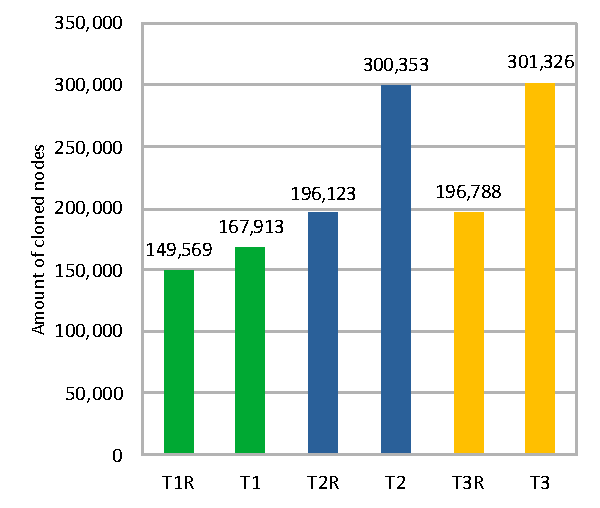
\includegraphics[width=\textwidth]{img/TypeResults}
    \caption{Number of cloned nodes.}
\label{fig:typeres}
  \end{minipage}
  \hfill
  \begin{minipage}[b]{0.45\textwidth}
    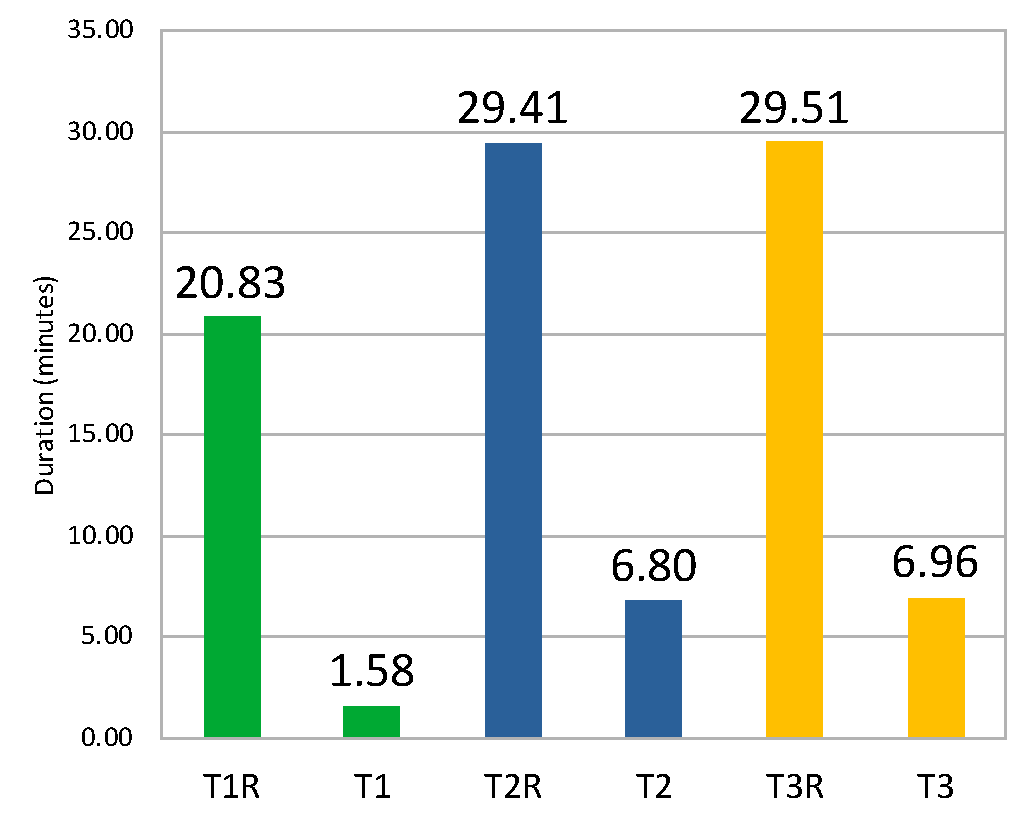
\includegraphics[width=\textwidth]{img/DurationChart}
    \caption{Clone type performance.}
  \label{fig:performance}
  \end{minipage}
\end{figure}
% Sander: korte uitleg over wat we zien in de figures hier? (geld voor alle experimenten)

\subsection{Performance}
To map the viability of refactoring-oriented clone types for large scale clone detection, we measured the duration of finding clones by the different clone types. Figure~\ref{fig:performance} shows the duration of detecting all clones in the corpus using CloneRefactor for different clone types. This figure shows the average duration of running CloneRefactor 10 times for a certain clone type. We ran these performance tests on the compute nodes of the DAS4 supercomputer \cite{bal2016medium}, which do not have many background processes severely affecting the results. % Sander: zou zin na de komma (which..results) weglaten.
The durations are of course dependent on our implementation of the clone types.
% Sander: deze zin voegt ook niet zoveel toe

\subsection{Type 2R Variability Threshold}
To determine the influence of the type 2R variability threshold on the amount of found nodes, we ran CloneRefactor for all variability percentages (0\% meaning no variance in expressions, 100\% meaning any variance in expressions). Figure \ref{fig:t2rgraph} shows the results.

\begin{figure}[H]
  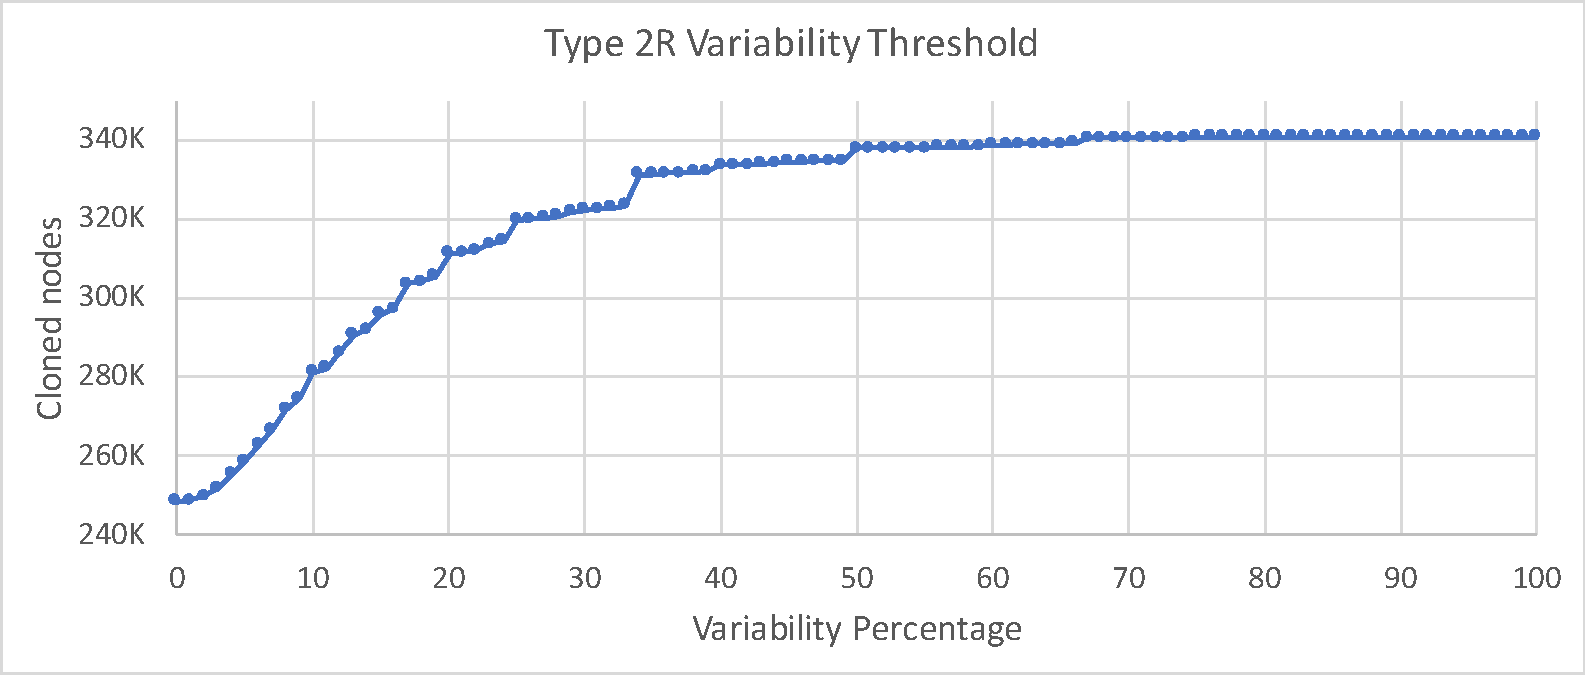
\includegraphics[width=1\textwidth]{img/T2R}
  \caption{Cloned nodes found for different Type 2R thresholds.}
  \label{fig:t2rgraph}
\end{figure}

\subsection{Type 3R Gap Size Thresholds}
To determine the influence of the type 3R gap size threshold on the amount of found nodes, we ran CloneRefactor for all gap size percentages between 0\% and 200\%. Figure \ref{fig:t3rgraph} shows the results.

\begin{figure}[H]
  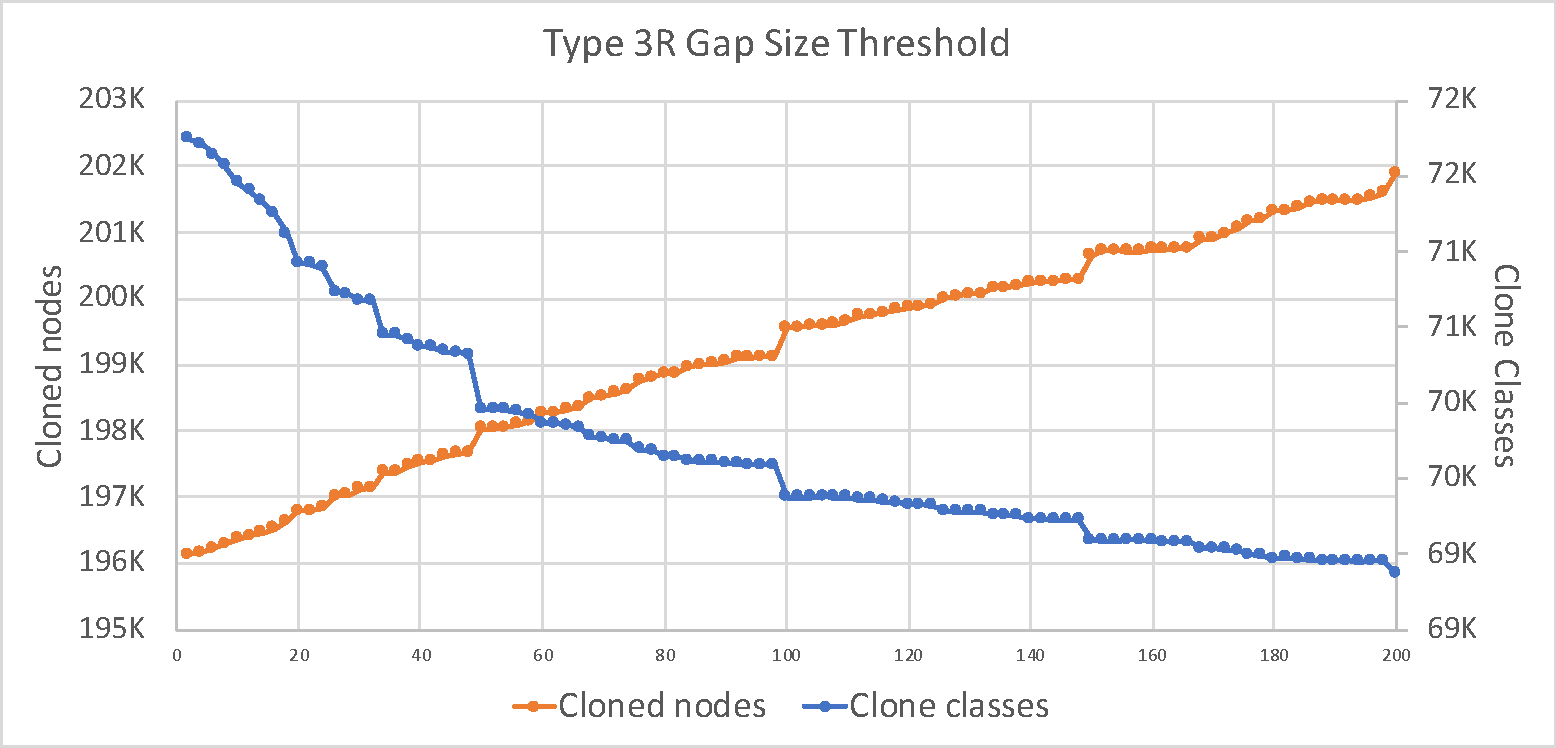
\includegraphics[width=1\textwidth]{img/T3R}
  \caption{Cloned nodes and clone classes found for different Type 3R thresholds.}
  \label{fig:t3rgraph}
\end{figure}

\section{Clone context}
% How many clones are there in certain contexts? Experiments for relation, location, and context.
To determine the refactoring method(s) that can be used to refactor most clones, we perform statistical analysis on the context of clones (see Section~\ref{chap:contextsetup}).

\subsection{Relation} \label{sec:relationresults}
Table~\ref{tab:relation} displays the number of clone classes found for the entire corpus for different relations (see Section~\ref{sec:setuprelation}).
% Sander: is dat plaatje met overzicht van relaties van clone classen weg of ergens anders? hij is hier ook wel handig

\begin{table}[H]
\centering
\begin{tabular}{@{}llllll@{}}
\toprule
\textit{\textbf{Category}} & \textit{\textbf{Relation}} & \textit{\textbf{Clone Classes}} & \textit{\textbf{\%}} & \textit{\textbf{Total}} & \textit{\textbf{\%}} \\ \midrule
\multirow{2}{*}{Common Class} & Same Class & 22,893 & 26.8\% & \multirow{2}{*}{31,848} & \multirow{2}{*}{37.2\%} \\ \cmidrule(lr){2-4}
 & Same Method & 8,955 & 10.5\% & & \\ \midrule
\multirow{5}{*}{Common Hierarchy} & Sibling & 15,588 & 18.2\% & \multirow{5}{*}{20,342}& \multirow{5}{*}{23.8\%} \\ \cmidrule(lr){2-4}
 & Superclass & 2,616 & 3.1\% & & \\ \cmidrule(lr){2-4}
 & First Cousin & 1,219 & 1.4\% & & \\ \cmidrule(lr){2-4}
 & Common Hierarchy & 720 & 0.8\% & & \\ \cmidrule(lr){2-4}
 & Ancestor & 199 & 0.2\% & & \\ \midrule
\multirow{4}{*}{Unrelated} & No Direct Superclass & 10,677 & 12.5\% & \multirow{4}{*}{20,314}& \multirow{4}{*}{23.7\%} \\ \cmidrule(lr){2-4}
 & External Superclass & 4,525 & 5.3\% & & \\ \cmidrule(lr){2-4}
 & External Ancestor & 3,347 & 3.9\% & & \\ \cmidrule(lr){2-4}
 & No Indirect Superclass & 1,765 & 2.1\% & & \\ \midrule
\multirow{2}{*}{Common Interface} & Same Direct Interface & 7,522 & 8.8\% & \multirow{2}{*}{13,074} & \multirow{2}{*}{15.3\%} \\ \cmidrule(lr){2-4}
 & Same Indirect Interface & 5,552 & 6.5\% & & \\ \bottomrule
\end{tabular}
\caption{Number of clone classes per clone relation}
\label{tab:relation}
\end{table}

\subsection{Location}
Table~\ref{tab:contents} displays the number of clone classes found for the entire corpus for different locations (see Section~\ref{sec:setuplocation}).
\begin{table}[H]
\centering
\begin{tabular}{@{}lll@{}}
\toprule
Category & Clone instances & \% \\ \midrule
Method Level & 232,545 & 78.43\% \\
Class Level & 50,402 & 17.00\% \\
Constructor Level & 10,039 & 3.39\% \\
Interface Level & 2,693 & 0.91\% \\
Enum Level & 788 & 0.27\% \\
\end{tabular}
\caption{Amount of clone instances with a certain location} % Sander: miss: Amount of clone instances per location category ofzoiets
\label{tab:location}
\end{table}

\subsection{Contents}
Table~\ref{tab:contents} displays the number of clone classes found for the entire corpus for different contents (see Section~\ref{sec:setupcontents}).

\begin{table}[H]
\centering
\begin{tabular}{@{}llllll@{}}
\toprule
\textit{\textbf{Category}} & \textit{\textbf{Contents}} & \textit{\textbf{Clone instances}} & \textit{\textbf{Total}} \\ \midrule
\multirow{2}{*}{Partial} & Partial Method & 219,540 & 74.05\% & \multirow{2}{*}{229,521}& \multirow{2}{*}{77.42\%} \\ \cmidrule(lr){2-4}
 & Partial Constructor & 9,981 & 3.37\% & & \\ \midrule
\multirow{5}{*}{Full} & Full Method & 12,990 & 4.38\% & \multirow{5}{*}{13,173}& \multirow{5}{*}{4,44\%} \\ \cmidrule(lr){2-4}
 & Full Interface & 64 & 0.02\% & & \\ \cmidrule(lr){2-4}
 & Full Constructor & 58 & 0.02\% & & \\ \cmidrule(lr){2-4}
 & Full Class & 37 & 0.01\% & & \\ \cmidrule(lr){2-4}
 & Full Enum & 24 & 0.01\% & & \\ \midrule
\multirow{3}{*}{Other} & Several Methods & 22,749 & 7.67\% & \multirow{3}{*}{53,773} & \multirow{3}{*}{18.14\%} \\ \cmidrule(lr){2-4}
 & Only Fields & 17,700 & 5.97\% & & \\ \cmidrule(lr){2-4}
 & Other & 13,324 & 4.49\% & & \\ \bottomrule
\end{tabular}
\caption{Number of clone instances for clone contents categories}
\label{tab:contents}
\end{table}

\section{Extract Method}
%To what extent can found clones be refactored through method extraction, without requiring additional transformations.
Table~\ref{tab:refactorability} shows to what extent clone classes can be refactored by using the ``Extract Method'' refactoring technique. The second column shows our measurements for the complete systems (just like the former experiments). The third column shows our measurements when restricting our search to method bodies. % Sander: waarom willen we dat weten?
The amount that can be extracted increases because, when restricting our search to method bodies, we do not exclude declarations that can obstruct the possibility of method extraction (for instance a cloned method signature).
% Sander: die laatste zin snap ik niet
\begin{table}[H]
\centering
\begin{tabular}{@{}lllll@{}}
\toprule
\textit{\textbf{Category}} & \textit{\textbf{All}} & \textit{\textbf{\% (All)}} & \textit{\textbf{Method Body}} & \textit{\textbf{\% (Method Body)}} \\ \midrule
Can Be Extracted & 24,157 & 28.2\% & 26,109 & 50.4\% \\
Is Not A Partial Method & 21,625 & 25.3\% & 0 & 0.0\% \\
Top-level AST-Node is not a Statement & 19,887 & 23.2\% & 4,607 & 8.9\% \\
Spans Part of a Block & 12,964 & 15.2\% & 13,460 & 26.1\% \\
Multiple Return Values & 5,622 & 6.6\% & 6,131 & 11.9\% \\
Complex Control Flow & 1,106 & 1.3\% & 1,216 & 2.4\% \\
Overlap In Clone Class & 147 & 0.2\% & 147 & 0.3\% \\
Not In Class Or Interface & 70 & 0.1\% & 93 & 0.2\% \\
\bottomrule
\end{tabular}
\caption{Number of clones that can be extracted using the ``Extract Method'' refactoring technique}
\label{tab:refactorability}
\end{table}

\section{Refactoring}
%I think the ultimate goal with this thesis is to do experiments with different clone thresholds. Which thresholds give clones that we should refactor? For this, we will measure the maintainability of the refactored source code over different thresholds. These thresholds range from minimum clone size, variability, and gap size.
In our corpus, CloneRefactor has refactored 12,710 clone classes and measured the change in indicated metrics (see Section~\ref{sec:metrics}). Using the presented formulas (see Section~\ref{sec:metricformula}) we determine how the characteristics of the extracted method (see Section~\ref{sec:characteristics}) % Sander: Ref geeft ???
influence the maintainability of the resulting codebase after refactoring. In this section, we explore the data received by comparing the before- and after snapshots of the system for each separate refactoring.

\subsection{Clone Token Volume}
Figure \ref{fig:maintainabilityscore} shows the obtained results when plotting the clone volume vs the maintainability increase/decrease. We define the \textit{token volume} as the combined number of tokens in all clone instances in a refactored clone class. The maintainability score, as shown in Figure \ref{fig:maintainabilityscore}, is the average delta maintainability score of all clone classes with the specified token volume that are refactored. As the amount of data points decreases, the datapoints gain less statistical significance, because of which we represent the x-axis as a logaritmic scale.% Sander: weet niet zeker of dit logaritmische schaal heet
The trendline intersects the ``zero'' line (maintainability does not increase nor decrease) at a token volume of 63.

\begin{figure}[H]
  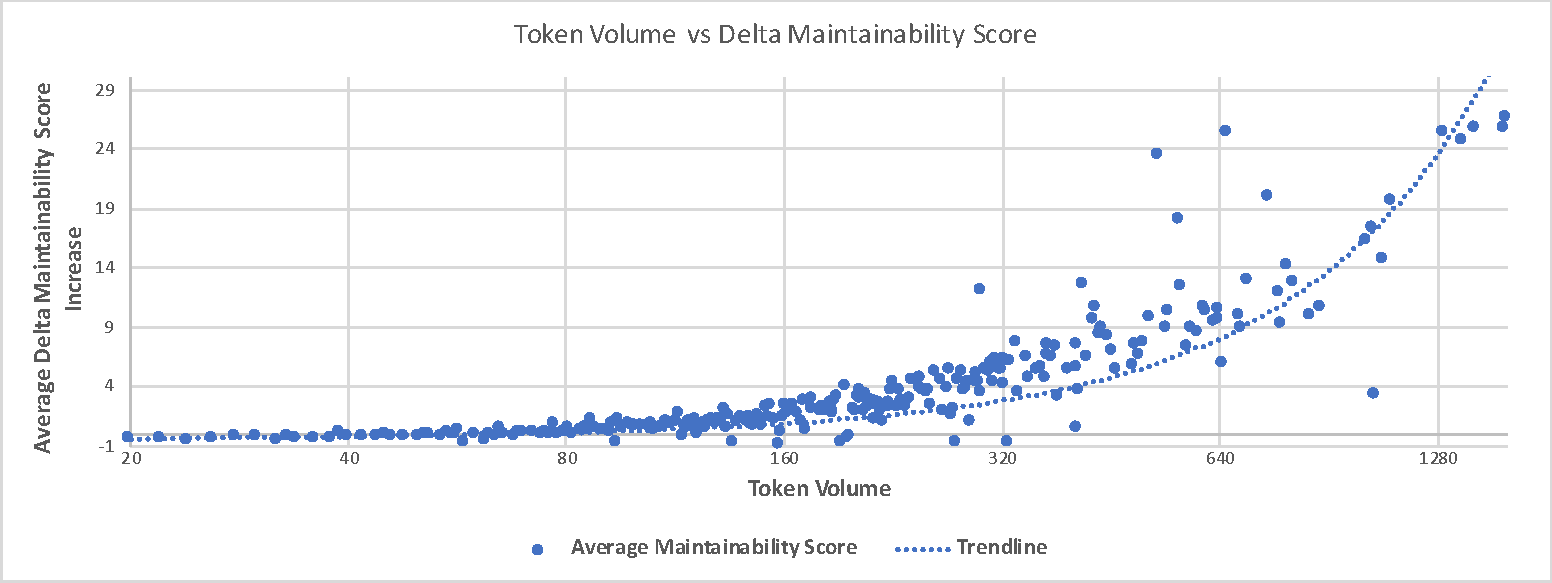
\includegraphics[width=1\textwidth]{img/maintainabilityscore}
  \caption{The effect of token volume on the delta maintainability score of the refactored clones}
  \label{fig:maintainabilityscore}
\end{figure}

The token volume of the clone is equal to the decrease of duplicated tokens, which is part of the maintainability score. Because of that, what we see in Figure~\ref{fig:maintainabilityscore} could largely be caused by this metric. Do determine the effect of clone token volume on each metric, we also plot graphs in which each metric is considered singularly. In Figure~\ref{fig:volume} the average delta volume is shown when clones with the specified token volume are refactored. The trendline intersects the ``zero'' line (average delta volume does not increase nor decrease) at 60 tokens. A higher average delta volume implies a lower maintainability.

\begin{figure}[H]
  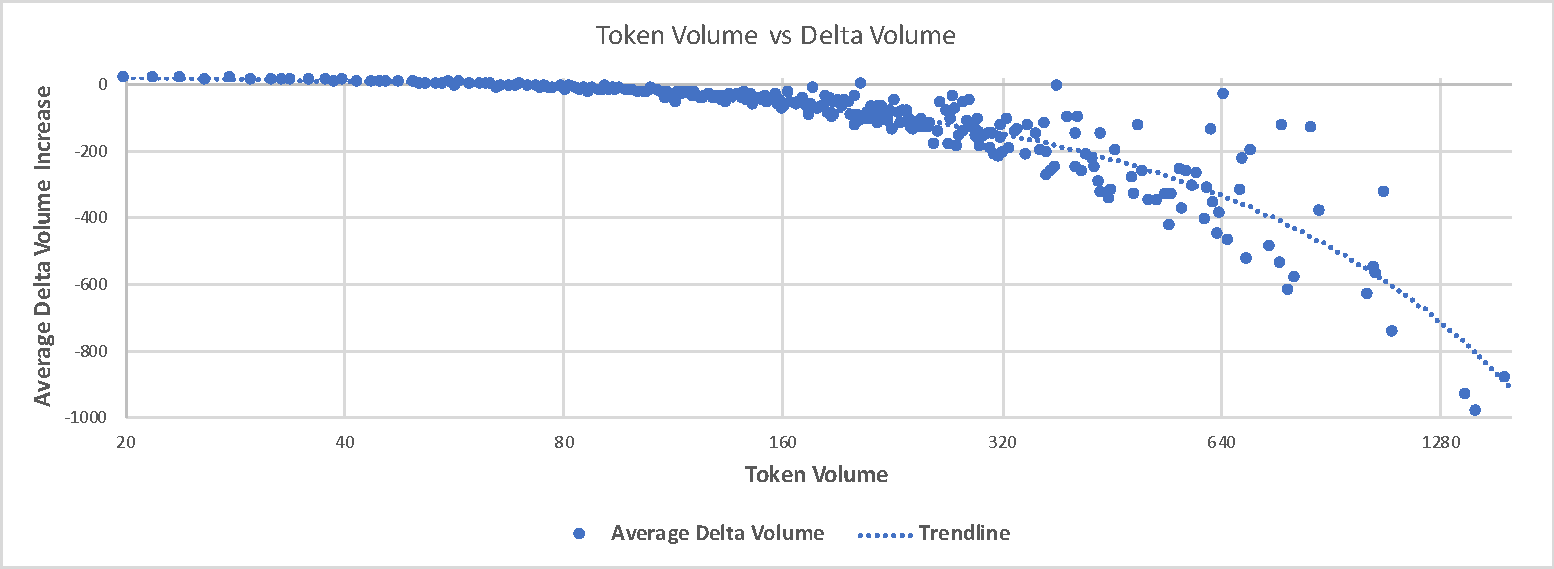
\includegraphics[width=1\textwidth]{img/volume}
  \caption{The effect of token volume on the delta volume of the refactored clones}
  \label{fig:volume}
\end{figure}

In Figure~\ref{fig:numberofparameters} we show the average delta number of parameters when clones with the specified token volume are refactored. This metric can only increase by the refactoring, because CloneRefactor only applies ``Extract Method'' refactorings that create a method with a certain number of parameters (according to the data needed by the extracted method).

\begin{figure}[H]
  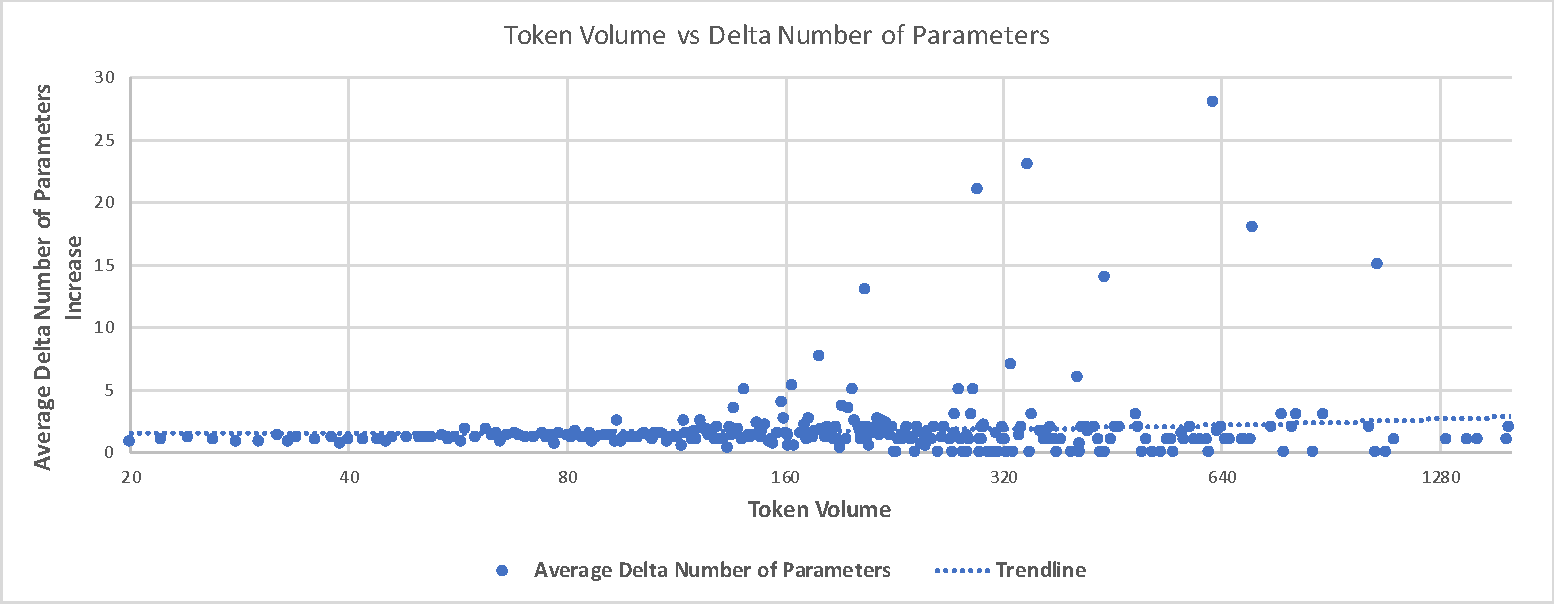
\includegraphics[width=1\textwidth]{img/numberofparameters}
  \caption{The effect of token volume on the number of parameters of the refactored clones}
  \label{fig:numberofparameters}
\end{figure}

In Figure~\ref{fig:complexity} we show the average delta complexity when clones with the specified token volume are refactored. We did not add a trendline, as there does not seem to be a clear trend. The maximum delta complexity is 1, because the extracted method itself has a complexity of 1. For each branching point in the cloned fragment, the complexity of the system will decrease when such a clone is refactored.

\begin{figure}[H]
  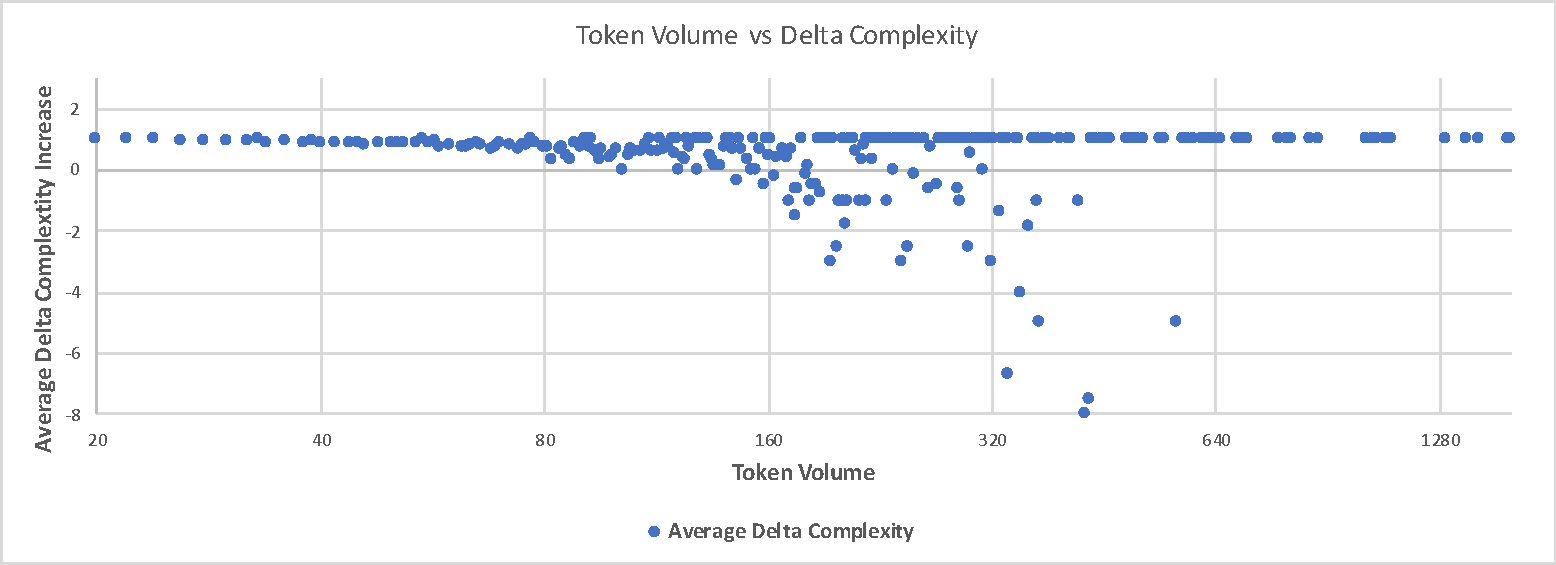
\includegraphics[width=1\textwidth]{img/complexity}
  \caption{The effect of token volume on the complexity of the refactored clones}
  \label{fig:complexity}
\end{figure}

%The volume of the clone is the dominating factor regarding the maintainability increase/decrease of cloned code. Because of that, in our further experiments we filter out all refactorings with a token size smaller than 18 because otherwise the small clones dominate the results and turn all results towards unmaintainable.

\subsection{Relation}
Table~\ref{tab:relation_refactor} shows our data regarding how different relations influence maintainability. We mark rows based on less than 100 refactorings red, as their result does not have statistical significance.

\begin{table}[H]
\centering
\begin{tabular}{@{}lll@{}}
\toprule
\textit{\textbf{Relation}} & \textit{\textbf{Maintainability Score}} & \textit{\textbf{Number of Refactorings}} \\ \midrule
\textbf{Common Hierarchy} & \textbf{0.23} & \textbf{2,202} \\ \midrule
\hspace{10pt} Superclass & 0.42 & 229 \\
\hspace{10pt} Sibling & 0.23 & 1,722 \\
\rowcolor[HTML]{FFCCC9}
\hspace{10pt} Same Hierarchy & 0.10 & 87 \\
\hspace{10pt} First Cousin & 0.02 & 144 \\
\rowcolor[HTML]{FFCCC9}
\hspace{10pt} Ancestor & -0.03 & 20 \\ \midrule
\textbf{Common Interface} & \textbf{-0.02} & \textbf{1,044} \\ \midrule
\hspace{10pt} Same Indirect Interface & -0.01 & 487 \\
\hspace{10pt} Same Direct Interface & -0.02 & 557 \\ \midrule
\textbf{Common Class} & \textbf{-0.02} & \textbf{7,239}\\ \midrule
\hspace{10pt} Same Class & 0.04  & 4,874 \\
\hspace{10pt} Same Method & -0.15 & 2,365  \\ \midrule
\textbf{Unrelated} & \textbf{-0.15} & \textbf{2,198}\\ \midrule
\hspace{10pt} No Direct Superclass & -0.06 & 811 \\
\hspace{10pt} External Superclass & -0.17 & 697  \\
\hspace{10pt} External Ancestor & -0.21 & 586  \\
\hspace{10pt} No Indirect Superclass & -0.30 & 104  \\ \midrule
\end{tabular}
\caption{Influence on maintainability of refactoring clones by certain relations.}
\label{tab:relation_refactor}
\end{table}

\subsection{Return Value}
Table~\ref{tab:return} shows how the return value of the extracted method influences the maintainability of the resulting system (categories are explained in Section~\ref{sec:refreturn}).

\begin{table}[H]
\centering
\begin{tabular}{@{}lll@{}}
\toprule
\textit{\textbf{Return Value}} & \begin{tabular}[c]{@{}l@{}}\textit{\textbf{Maintainability}}\\\textit{\textbf{Score}}\end{tabular} & \begin{tabular}[c]{@{}l@{}}\textit{\textbf{Number of}}\\\textit{\textbf{Refactorings}}\end{tabular} \\ \midrule
Return & 0.19 & 1,571 \\
Declare & 0.15 & 5,177 \\
\rowcolor[HTML]{FFCCC9}
Assign & 0.12 & 14 \\
Void & -0.18 & 5,921 \\
\bottomrule
\end{tabular}
\caption{Maintainability scores for different methods of handling returned data from the call to the extracted method.}
\label{tab:return}
\end{table}

\subsection{Parameters}
Fig.~\ref{fig:arguments} shows how an increase in parameters lowers the maintainability of the refactored code. On the primary x-axis, the maintainability is displayed. The secondary x-axis shows the number of refactorings. The y-axis shows the number of parameters.

\begin{figure}[H]
  \centering
  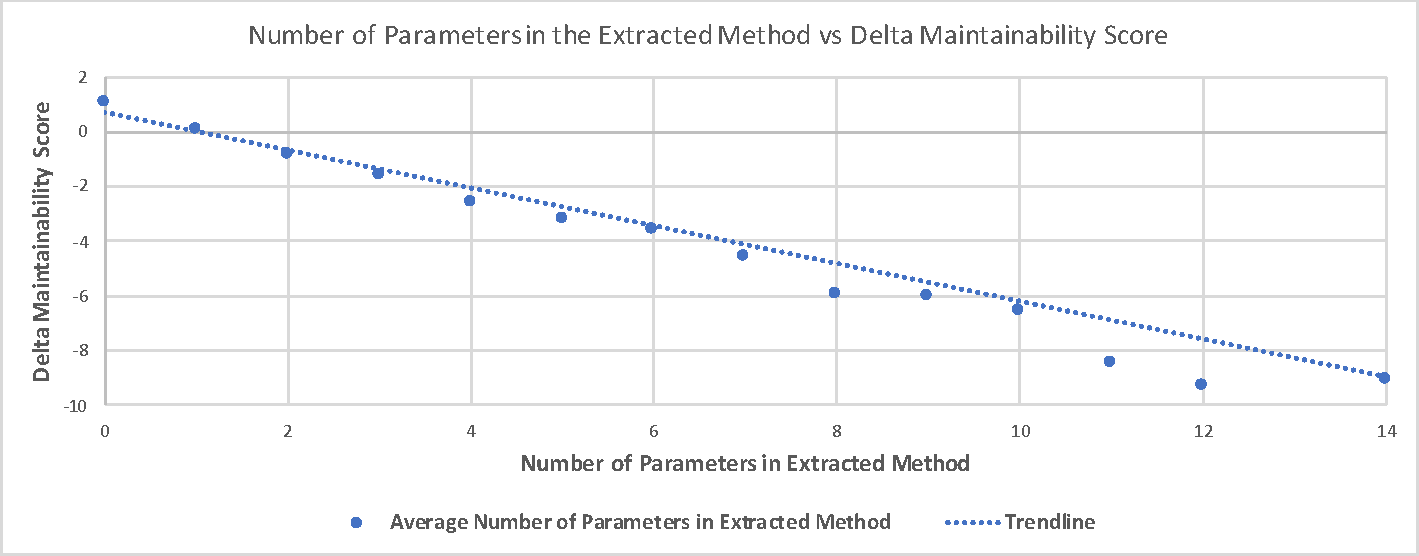
\includegraphics[width=0.8\columnwidth]{img/arguments}
  \caption{Influence of number of method parameters on system maintainability.}
  \label{fig:arguments}
\end{figure}
